\chapter{Project Plan}
\label{ch:project_plan}
In the following section, the project plan of the proposed master's thesis is discussed.
The project plan consists of a work plan, time schedule, and risk assessment.
The work plan defines the project objectives, milestones, tasks, and deliverables and is presented in \autoref{sec:work_plan}.
The time schedule represents the mapping of the proposed work plan to calendar weeks and is discussed in \autoref{sec:time_schedule}.
The risk assessment evaluates technical and non-technical risks for the proposed project plan and is discussed in \autoref{sec:risk_assessment}.

\section{Work Plan}
\label{sec:work_plan}
%\todo{Workplan, Incremental Parts ("inkremente"), Dependencies, Deliverable-Duration-Limitation, time schedule (milestones, temporal dependencies)}
The work plan structures the proposed thesis into six milestones.
Each milestone represents a major phase of the proposed master's thesis.
The milestones serve as intermediate project goals which enable monitoring and reporting of project progress.
Each milestone is defined by its starting date, duration in calendar weeks (CW), and deliverables.
Moreover, each milestone consists of at least one task.
The tasks of a milestone are referred to as increments.
The milestones of the proposed master's thesis are defined as follows:
\begin{description}
    \item[Milestone I:] Preliminary Work
    \begin{description}[style=multiline, leftmargin=\widthof{\textbf{Deliverables:}}]
        \item[Duration:] 14 Weeks (15. April 2024 (CW 16) -- 22. July 2024 (CW 30))
        \item[Deliverables:] Master's thesis proposal
    \end{description}
    \item[Milestone II:] Realization
    \begin{description}[style=multiline, leftmargin=\widthof{\textbf{Deliverables:}}]
        \item[Duration:] 9 Weeks (22. July 2024 (CW 30) -- 23. September 2024 (CW 39))
        \item[Deliverables:]
        \begin{enumerate}[label=\alph*), leftmargin=\widthof{a)}+\labelsep]
            \item Software Design, Implementation, Tests (Unit, Integration, and System), \& Test Coverage Report of CASC-SAS
            \item Hardware Deployment Scripts of CASC-SAS
            \item Thesis Chapter: Realization
        \end{enumerate}
        \item[Increments:]
        \begin{enumerate}[label=\arabic*), leftmargin=\widthof{a)}+\labelsep]
            \item Design, Implementation, Tests, \& Deployment of CASA (8 Weeks)
            \item Design, Implementation, Tests, \& Deployment of SABAAC (8 Weeks)
            \item Architecture \& Code Review (Optional, Single Meeting)
            \item Writing of Documentation (5 Weeks)
        \end{enumerate}
    \end{description}
    \item[Milestone III:] Evaluation
    \begin{description}[style=multiline, leftmargin=\widthof{\textbf{Deliverables:}}]
        \item[Duration:] 9 Weeks (23. September 2024 (CW 39) -- 25. November 2024 (CW 48))
        \item[Deliverables:]
        \begin{enumerate}[label=\alph*), leftmargin=\widthof{a)}+\labelsep]
            \item Evaluation Results of CASC-SAS
            \item Thesis Chapter: Evaluation
        \end{enumerate}
        \item[Increments:]
        \begin{enumerate}[label=\arabic*), leftmargin=\widthof{a)}+\labelsep]
            \item Security Evaluation (9 Weeks)
            \item Performance Evaluation (9 Weeks)
            \item Economic Evaluation (5 Weeks)
            \item Writing of Documentation (4 Weeks)
        \end{enumerate}
    \end{description}
    \item[Milestone IV:] Conclusion
    \begin{description}[style=multiline, leftmargin=\widthof{\textbf{Deliverables:}}]
        \item[Duration:] 2 Weeks (25. November 2024 (CW 48) -- 09. December 2024 (CW 50))
        \item[Deliverables:]
        \begin{enumerate}[label=\alph*), leftmargin=\widthof{a)}+\labelsep]
            \item Thesis Chapter: Conclusion
            \item Thesis Chapter: Limitations
            \item Thesis Chapter: Future Work
            \item Thesis Chapter: Abstract
        \end{enumerate}
        \item[Increment:] Writing of Documentation: Conduct a review of results and derive a conclusion, limitations, and future work with regard to the research questions (2 Weeks)
    \end{description}
    \item[Milestone V:] Review
    \begin{description}[style=multiline, leftmargin=\widthof{\textbf{Deliverables:}}]
        \item[Duration:] 5 Weeks (09. December 2024 (CW 50) -- 13. January 2025 (CW 03))
        \item[Deliverables:] Reviewed \& Proofread Master's Thesis
        \item[Increments:]
        \begin{enumerate}[label=\arabic*), leftmargin=\widthof{a)}+\labelsep]
            \item Internal Review: Proofreading \& Correction by the Authors (2 Weeks)
            \item External Review: Proofreading \& Correction by External Readers (4 Weeks)
        \end{enumerate}
    \end{description}
    \item[Milestone VI:] Finalization
    \begin{description}[style=multiline, leftmargin=\widthof{\textbf{Deliverables:}}]
        \item[Duration:] 6 Weeks (09. December 2024 (CW 50) -- 20. January 2025 (CW 04))
        \item[Deliverables:]
        \begin{enumerate}[label=\alph*), leftmargin=\widthof{a)}+\labelsep]
            \item Printed \& Bound Master's Thesis
            \item Master's Thesis Presentation Slides
        \end{enumerate}
        \item[Increments:]
        \begin{enumerate}[label=\arabic*), leftmargin=\widthof{a)}+\labelsep]
            \item Thesis Presentation Preparation (5 Weeks)
            \item Printing \& Binding of Thesis (1 Weeks)
        \end{enumerate}
    \end{description}
\end{description}

\section{Time Schedule}
\label{sec:time_schedule}
\dots
\begin{figure}
    \centering
    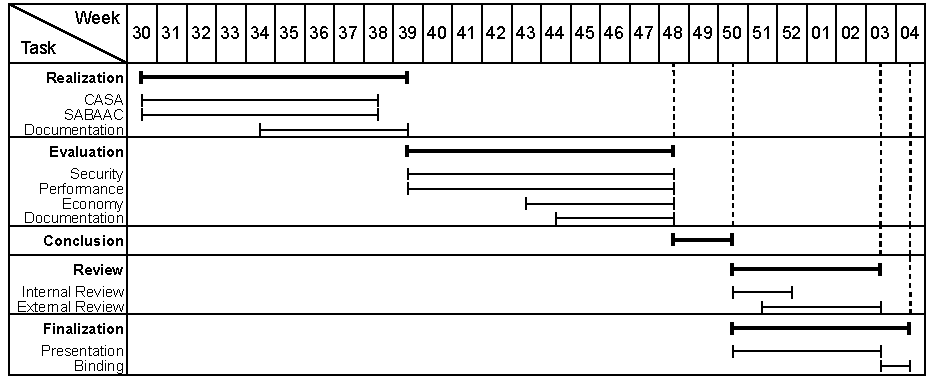
\includegraphics[width=1.0\linewidth]{figures/timeplan.drawio.pdf}
    \caption{Time schedule of the proposed master's thesis.}
    \label{fig:timeplan}
\end{figure}

\section{Risk Assessment}
\label{sec:risk_assessment}
The risk assessment identifies technical as well as project management risks and assesses their impact on the proposed project plan.\dots
\todo{Find, analyse, describe, estimate risks}
\todo{Provide mitigation ideas for each risk}
